\documentclass[a4paper, amsfonts, amssymb, amsmath, reprint, showkeys, nofootinbib, twoside]{revtex4-1}
\usepackage[english]{babel}
\usepackage[utf8]{inputenc}
\usepackage[colorinlistoftodos, color=green!40, prependcaption]{todonotes}
\input{preamble}
\usepackage[pdftex, pdftitle={Article}, pdfauthor={Author}]{hyperref} % For hyperlinks in the PDF
%\setlength{\marginparwidth}{2.5cm}
\bibliographystyle{apsrev4-1}
\usepackage{array}

\begin{document}
%\title{\textcolor{red}{Design strategies for the self-assembly of polyhedral shells using SAT-assembly}}
\title{\textcolor{red}{Design strategies for the self-assembly of polyhedral shells}}

\author{Diogo E. P. Pinto$^1$, Petr $\check{\text{S}}$ulc$^2$, Francesco Sciortino$^1$ and John Russo$^1$}
    \email[Correspondence email address: ]{john.russo@uniroma1.it}% Your name
    \affiliation{$^1$Dipartimento di Fisica, Sapienza Universit\`{a} di Roma, P.le Aldo Moro 5, 00185 Rome, Italy}
    \affiliation{$^2$School of Molecular Sciences and Center for Molecular Design and Biomimetics, The Biodesign Institute, Arizona State University, 1001 South McAllister Avenue, Tempe, Arizona 85281, USA}

\date{\today} % Leave empty to omit a date

\begin{abstract}
\textcolor{red}{The control over the self-assembly of complex structures is a long-standing challenge of material science, especially on the colloidal scale, as the desired assembly pathway is often kinetically derailed by the formation of amorphous aggregates. Here we investigate in detail the problem of the self-assembly of
%the
three Archimedean shells,
%that can be assembled from five-coordinated unit, 
i.e. the icosahedron, the snub cube, and the snub dodecahedron. We use Patchy Particles with five interaction sites (or patches) as our model for the building blocks, and recast the assembly problem as a satisfiability problem (SAT) for the patch interactions. This allows us to find effective designs for all targets, and to selectively suppress unwanted structures.
By tuning the geometrical arrangement and the specific interactions of the patches, we find 
that lowering the symmetry of the building blocks is an effective way to reduce the number of competing structures, which in turn can considerably increase the yield of the target structure. We also consider the concentration dependence of our assemblies as a way to externally control which target structure is formed.} These results cement SAT-assembly as an invaluable tool to solve inverse design problems.
\end{abstract}

\maketitle

\section{Introduction}

%The assembly of complex structures has been a longstanding challenge of material science \cite{Bishop2022}.
Self-assembly encompasses a large array of phenomena through which materials are formed using simple assembly rules of microscopic building blocks \cite{Whitelam2015}. In Nature, many striking examples of this assembly are found \cite{Whitesides2002, Parnell2015, Teyssier2015}. In the case of synthetic materials, although quite a complex process, some realizations have been successfully assembled, from three-dimensional crystals to polyhedral shells \cite{Dziomkina2005, Glotzer2007, Kim2011, LaCour2022,  McGorty2010, Mu2022, Nykypanchuk2008, Sacanna2011, Wang2012, Wang2015, Joshi2016,Bishop2022}. One of the main difficulties resides in how to optimize the geometrical properties or interactions between the building blocks without leading to a kinetically arrested configurations~\cite{Frenkel2011, Lash2015, Blaaderen2006, Meulen2015}.

\textcolor{red}{Here we focus on the self-assembly of finite-size structures and in particular on specific polyhedron shells. 
From an application standpoint, the potential of closed shells} to act as drug delivery systems have been a widely researched topic, where a given drug is encapsulated within a closed shell and then driven to a specific diseased area where the drug is locally released such that the least amount of non diseased tissue is affected \cite{Huang2007, Uchida2007}. For this, the shell needs to close around a specific reagent and then open when external conditions are met. Recently, there have been suitable experimental realizations, for example, using DNA-origami, where selective interactions can be introduced to mimic patchy particles \cite{Mosayebi2017, Lee2022, Jun2021, Rothemund2006}.

\textcolor{red}{When focusing on finite-size shells additional challenges arise compared to the ones encountered in the self-assembly of crystal structures. Firstly, the self-assembly occurs exclusively from the gas phase, which rules out the possibility to use (critical point induced) density fluctuations to accelerate the rate of aggregation, as frequently done in the case of crystals. On the contrary, the formation of finite-size aggregates stabilizes the gas phase to high densities with respect to the liquid phase, possibly introducing a density dependence of the aggregation pathway. Secondly, the small size of the aggregates, compared to the infinitely repeating units of a crystal, can stabilize kinetic straps, i.e. structures whose free-energy is not as low as the one of the target structure, but that requires an exceedingly long waiting time to break. Lastly, the formation of finite-size aggregates is a continuous process, and is not accompanied by a phase transition as in crystals. The absence of a critical-size of formation (i.e. the critical nucleus) means that it is not sufficient to suppress a handful of competing structures at one length-scale, but that the assembly process has to proceed without defects at every stage. This problem is reflected in the difficulty of perfectly closing large-size aggregates, such as capsids~\cite{Mosayebi2017}.}


\textcolor{red}{To tackle these challenges, we explore the inverse design of finite-size structure via a novel technique, named SAT-assembly\cite{Romano2020a,Russo2022}}. By describing the assembly as a constraint satisfiability problem (SAT), one is able to apply general tools to target the desired structures and exclude competing ones. One of its most successful applications is found in the design of patchy particles, where the building blocks are considered hard spheres with attractive patches on its surface \cite{Bianchi2006, Romano2010, Rovigatti2018, Russo2021, Sciortino2009}. These represent a coarse-grained approach to describe multiple systems, e.g. colloids, proteins, polymers, etc \cite{Sacanna2011, Wang2012}. If to each patch is associated a color, one can formulate a problem with boolean variables which translates into a particle design (patch colors of a given particle, color-color interactions, etc.). One can then create an array of constraints that enforce the topology of a given target structure onto these variables~\cite{Russo2022} \textcolor{red}{ and use a SAT solver~\cite{Een2005} to efficiently find a design which satisfies the constraints imposed.}
\textcolor{red}{Another key advantage of SAT-assembly is that it doesn't require geometrical intuition on the target structure~\cite{rapaport2004self}}.


\textcolor{red}{So far, SAT-assembly has been used to study the assembly of complex crystals, with an emphasis on structures that have photonic applications, such as the tetrastack~\cite{Romano2020a} and diamond cubic crystal~\cite{Romano2020a,Russo2022,rovigatti2022simple}, or structures with a high number of atoms in the unit cells, such as clathrate crystals~\cite{Romano2020a}. In this article we will show that SAT-assembly can be successfully can be used to tackle the problem of assembling finite-size structures, opening the doors for a robust assembly process where one can avoid competing polyhedra and make sure that a given design leads to the targeted shell.}


In this work we focus on patchy particles with a valence of 5 (number of patches on the surface of the sphere) and explore how one can tackle the problem of finite size assembly using SAT. We start by discussing the patchy particle model used and how SAT is applied to it. Then we describe the finite size shells found using an almost trivial solution given by SAT and how to control the geometrical and interaction parameters to bias the different configurations. We then discuss the thermodynamics of these systems and its critical miscel concentration. Finally we conclude by showing how to push SAT to target, in an efficient way, a given polyhedron shell. We conclude with a discussion and an outlook.

\section{Model}

We consider a system composed of $N$ patchy particles in a cubic box of length $L$. The particles are characterized by a hard core of radius $\sigma$ with five patches on its surface. The patches interact through the Kern-Frenkel portential \cite{Kern2003}:

\begin{equation}
Vpp(\boldsymbol{r}_{ij}, \boldsymbol{\hat{r}}_{\alpha, i}, \boldsymbol{\hat{r}}_{\beta, j})=V_{SW}(r_{ij})f(\boldsymbol{r}_{ij}, \boldsymbol{\hat{r}}_{\alpha, i}, \boldsymbol{\hat{r}}_{\beta, j})
\end{equation}

where $i$ corresponds to a given particle and $\boldsymbol{r}_{i}$ its center of mass. Thus, $\boldsymbol{r}_{ij}$ is the distance between particles $i$ and $j$. $\boldsymbol{r}_{\alpha, i}$ denotes the position of patch $\alpha$ of particle $i$. $V_{SW}$ is an isotropic square-well of range $\sigma + \delta_{\alpha,\beta}$ and depth $\varepsilon_{\alpha,\beta}$, the hat symbol indicate unit vectors and $f$ is the orientation-dependent modulation term that takes the form:

\begin{equation}
\label{KF}
f(\boldsymbol{r}_{ij}, \boldsymbol{\hat{r}}_{\alpha, i}, \boldsymbol{\hat{r}}_{\beta, j})=
    \begin{cases}
        1 & \text{if $\begin{aligned}
            \text{$\boldsymbol{\hat{r}}_{ij} \cdot \boldsymbol{\hat{r}}_{\alpha, i} > \cos     \theta^{max}_{\alpha \beta}$} \\
            \text{$\boldsymbol{\hat{r}}_{ji} \cdot \boldsymbol{\hat{r}}_{\beta, j} > \cos     \theta^{max}_{\alpha \beta}$}
        \end{aligned}$ } \\
        0 & \text{otherwise}
    \end{cases}
\end{equation}

With this formulation patches are represented by a cone starting from the center of mass of the particle and reaching $\sigma + \delta_{\alpha,\beta}$, while the width is controlled by $\theta^{max}_{\alpha \beta}$. This potential has been extensively used to study systems of patchy particles \cite{Rovigatti2018}. For simplicity, we consider the parameter range where it is only possible to form one bond per patch. In the following, $\sigma$ provides the unit of length and $\varepsilon_{\alpha, \beta}$ the unit of energy. Temperature ($T$) is also expressed in units of $\varepsilon_{\alpha, \beta}$ and $k_B=1$.

For the following results we considered Monte Carlo (MC) simulations with two possible moves, rototranslations and aggregation-volume-bias. The first attempts a simple rotation and translation of a random particle along a random (radial or angular) direction. The second, attempts to move a random particle into the vicinity of another such that a bond is formed between the two. To not break ergodicity, the inverse move can also be performed where a random bond between two particles is broken. We performed simulations in the $NVT$ assemble to explore the assembly of our desired shells. All results shown bellow were averages over simulations with or more than $10^8$ MC time-steps. For all, we considered $N=480$ and $\delta_{\alpha, \beta}=0.2$. The simulations start with particles randomly generated in the box with random orientations. Unless stated otherwise, all results are averages over $10$ independent samples.

We follow the same SAT formulation as the one in Ref.~\cite{Russo2021}. We consider that each patch can have a given color between $1\leq x_c\leq N_c$, where $N_c$ is the total number of colors. These colors can be distributed onto the patches in specific arrangements, each unique sequence can be considered a particle specie, thus $1\leq x_p\leq N_p$, where $N_p$ is the total number of species. SAT is then used to find if a given combination of $N_p$ and $N_c$ can satisfy a given polyhedral shell, e.g. if it satisfies all the topological constraints, and a solution/design is calculated which can be used to prepare the composition of the system. In the \emph{Supplemental Material} we go into more detail on the different constraints (clauses) used in SAT.

In Fig~\ref{SAT} we have a schematic showing the patchy particles used and the different configurations assembled. There are three possible polyhedron shells that can form and fully close, depending on the parameters and SAT solution used: the regular icosahedron, the snub cube and the snub dodecahedron. We consider the assembly of patchy particles of valence five. The positions of the patches, in the orthonormal base associated with the patchy particle, are given as:

\begin{equation}
    \label{patch}
    \begin{aligned}
    \textbf{p}_1=(-0.698, 0.186, -0.691) \\
    \textbf{p}_2=(-0.502, -0.756, -0.419) \\
    \textbf{p}_3=(-0.123, -0.857, 0.5) \\ 
    \textbf{p}_4=(-0.410, -0.007, 0.912) \\
    \textbf{p}_5=(-0.751, -0.627, 0.204) .
    \end{aligned}
\end{equation}

\noindent for the case of the icosahedron. To form the other structures one can increase the in plane angle between $\textbf{p}_4$ and $\textbf{p}_5$ while maintaining the remaining ones. In the next section we explore how this geometrical change plays a role in the assembly. We look at different in plane angles between these two patches ranging from the minimum of $60$ degrees, for the icosahedron, to the maximum of $108$ degrees, for the snub dodecahedron.

Using SAT we can find a minimal design that satisfies all three structures. For example, it is possible to consider the case that is shown in Fig.~\ref{SAT}, where we only use one specie (blue) of particles and two colors (green and red) for patches. In this design, green patches only interact with green and red with red. If the particles follow this coloring and interactions then the three structures can form. The SAT solution that leads to this design is not necessarily the only one that satisfies all structures but SAT only provides one solution at a time for the constraints provided. Nonetheless, it is flexible enough, such that, we can provide this solution found as a new constraint and thus avoid it altogether leading to new solutions (translating into different particle designs). This process can be iterated until all solutions are exhausted. We will first focus on this design with one specie and two colors to explore how the interaction and geometry of the patches plays a role in the assembly. We will also use it to explore the phase behavior of this patchy particle system. Then, we will use SAT to target specific shells in order to highlight the true use of SAT as a robust predicting tool.

\begin{figure}[t]
	\includegraphics{fig1.pdf}
	\caption{\label{SAT} Schematic representation of the structures explored. A particle with valence 5 is used to assemble the different polyhedron shells. A solution calculated with SAT is used for the patchy particle design which satisfies all three structures. It contains only one particle specie (blue) and two patch colors (green and red). The green patches only interact with green while the red only interact with red.}
\end{figure}

\section{Results}

As a first approach to the assembly problem posed in Fig.~\ref{SAT}, we consider the most trivial design possible: one particle specie and one patch color. Due to its simplicity we do not require the help of SAT to design the patchy particles. Using the simulation scheme detailed in the previous section we explore different values of the patch width, $\cos\theta_{max}$ (in Eq.~\ref{KF}, where we drop $\alpha$ and $\beta$ for simplicity) as well as different geometries of the patches by changing the in plane angle created by $\textbf{p}_4$ and $\textbf{p}_5$ in Eq.~\ref{patch}. The former allows for more flexibility of the bonds due to larger patch widths. The latter improves our ability to target the different structures proposed in Fig.~\ref{SAT} by more easily satisfying their geometry. For example, if the in plane angle between these vectors is close to $90$ degrees it is easier to form the squares in the snub cube.

\subsection{One particle specie designs}

Figure \ref{N1c1} shows the results measured for the trivial solution. It shows the most probable structure found out of the ones shown in Fig.~\ref{SAT}. If none of them is formed then we classify the clusters into two groups. The black crosses correspond to incomplete clusters, the ones where particles form bonds but they do not close, thus forming an open shell. The gray stars correspond to irregular aggregates, thus clusters that form and are able to completely close but are none of the ones in Fig.~\ref{SAT}. They are irregular in the sense that they do not correspond to any specific polyhedron. We find that only the icosahedron is able to form for the range of parameters explored. Furthermore, increasing patch width (lowering $\cos\theta_{max}$), thus increasing bond flexibility hinders the assembly of these structures. We can conclude that it is not sufficient for a particle and patch design to satisfy the targeted structure for it to assemble.

\begin{figure}[t]
	\includegraphics{fig2.pdf}
	\caption{\label{N1c1} Most probable structure formed for different in plane angles of $\textbf{p}_4$ and $\textbf{p}_5$ in Eq.~\ref{patch} and for different patch width, $\cos\theta_{max}$, in Eq.~\ref{KF}. The triangles inside the red region represent parameters where the most probable polyhedron shell from the ones in Fig.~\ref{SAT} is the icosahedron. Black crosses represent systems where open/incomplete clusters are more probable. The gray stars represent systems where clusters are able to close but none correspond to the ones in Fig.~\ref{SAT}. We find that for the most trivial solution only the icosahedron is able to form.}
\end{figure}

We now consider a non trivial design but with minimal colors and species. We use SAT to calculate a solution that satisfies all three structures but with only one particle specie and two patch colors, as shown in Fig.~\ref{SAT}. This solution dictates the patch design (which color has a given patch) and the interactions, which in this case are all self-similar (red with red and green with green). In Fig.~\ref{N1c2} are the results accompanied by some snapshots. Using this design we can identify the three different structures from Fig.~\ref{SAT} within the parameters explored. Examples are shown with the snapshots of the system. Thus, one can significantly improve on the trivial solution by using SAT as a design tool to assemble finite-size shells, even with minimal colors and species. These results also suggest that as patch width increases, structures with fewer particles are favored. Since the icosahedron requires less particles to form, the patch width compensates for the change in geometry (in plane angle of the patches).

\begin{figure}[t]
	\includegraphics{fig3.pdf}
	\caption{\label{N1c2} Most probable structure formed for different in plane angles of $\textbf{p}_4$ and $\textbf{p}_5$ in Eq.~\ref{patch} and for different patch width, $\cos\theta_{max}$, in Eq.~\ref{KF}. The triangles inside the red region represent parameters where the most probable structure from the ones in Fig.~\ref{SAT} is the icosahedron. The squares inside the green region represent parameters where the most probable structure from the ones in Fig.~\ref{SAT} is the snubcube. The pentagons inside the blue region represent parameters where the most probable structure from the ones in Fig.~\ref{SAT} is the snub dodecahedron. Black crosses represent systems where open/incomplete clusters are more probable. The gray stars represent systems where clusters are able to close but none correspond to the ones in Fig.~\ref{SAT}. On top of the plot are schematics of three different particles with the corresponding colors. The left one has an in plane angle of $60$ degrees, the middle of $90$ degrees and the right one of $108$ degrees. On the bottom are typical configurations from the parameters that are encircled in the plot. They were imaged with OVITO and the colors represent different clusters. The design used was of one specie and two colors, where all interactions are self-similar (red with red and green with green).}
\end{figure}

Figure \ref{Yield} shows the different yields of the polyhedron shells using the most optimized in plane angle for each ($60$ degrees for the icosahedron, $90$ degrees for the snub cube and $108$ degrees for the snub dodecahedron). We define the yield as the probability of finding a cluster corresponding to a specific structure. We count single particles as a cluster of size one and any bonded particles as clusters of size two or above, depending on the number of particles bonded. We find that for this design, C2(1), the snub cube has the highest yield for all the densities explored except the last one. We also observe that large structures like the snub dodecahedron, which is composed of $60$ particles, is more easily assembled in very dilute systems where larger shells have more space to grow without influencing each other. The fact that the yield of the snub cube is higher than the icosahedron, even though its shell is larger, is probably due to the specific design used. In the case of the snub cube, the patchy particle geometry is already asymmetrical and the solution used helps enforce it in the assembly, thus the clusters that are not snub cubes are incomplete shells. On the other hand, the icosahedron patchy particle has some rigid body rotational symmetries. For example, if every patch has the same color, one can rotate each particle as a rigid body four times while still satisfying the same topology. In the design with two colors, this symmetry is lost. For the particles to satisfy the topology of the assembly, each needs to have specific orientation, thus losing the rigid body rotational symmetry given by the patch positions. This leads to many clusters which are formed with twelve particles (the number of particles in the icosahedron) but with one or two bonds missing for it to fully close. 

In the same plots we show multiple other designs with only one specie, ranging from two colors to five. We find that, generally, the yield increases with the number of colors. At five colors the yield of the icosahedron and snub cube structures is close to maximum. This is due to the fact that the probability of creating a wrong bound decreases with increasing number of colors. For example, for the snub cube, there is only one specific bound that each patch can make in the final structure (since there is no rigid body rotational symmetry of the particles), but in the C2(1) case the top patches can form three possible connections. As such, the probability that the top three green patches form a correct bond is one third, while the two red bottom ones is one half. Thus, the probability of correctly assembling a particle is approximately $0.009$. As the number of colors increases so does the probability that a bond is formed correctly. For example, for the five colors there is only one possible bond formed for each patch (due to the interactions chosen) which is always the correct one. Thus, a particle can never form an incorrect bond. The only cases that do not follow this rule are the C2(1) and C2(2) designs. They share the same number of colors and are designed such that the probability of correct bonding is equal. Nonetheless, the average yield of the snub cube increases (from $\approx55\%$ to $\approx80\%$). We hypothesize that the design C2(2) creates a larger distinction between the patches than C2(1). In the case of the snub cube, the top three patches form the triangles seen in Fig.~\ref{SAT} while the two bottom patches form the square. In the design C2(1) the top three patches are indistinguishable, while in C2(2) its only a top one and the bottom two. Thus, in C2(2) the three top patches are now distinguishable by color while the bottom are by geometry. We hypothesize that this provides an easier pathway to assembly. The same is observed in the case of the snub dodecahedron, where now the bottom patches form pentagons. This is also supported by the fact that for the icosahedron, where all angles are the same, both designs have similar yields.

In the bottom right plot of Fig.~\ref{Yield} we observe how the yield changes as a function of a wider range of densities for $T=0.1$ using the five color design (C5). Using an intermediate in plane angle ($85.26$ degrees), we find that it is possible to change between the most probable structure formed by tuning the density of the system. For lower densities, the snub cube is more probable while for higher densities the icosahedron becomes more probable. Thus, these designs can be an ideal strategy to target different shells by only changing the system properties and keeping the design the same. This is useful for experiments where making particles with different functionalizations is a difficult task.

\begin{figure*}[t]
	\includegraphics{fig4.pdf}
	\caption{\label{Yield} Average yield of the icosahedron, snub cube and snub dodecahedron (in Fig.~\ref{SAT}) as a function of the density of patchy particles (Top right, top left and bottom left plots respectively). These results were calculated with $\cos\theta_{max}=0.98$ and the in plane angle was chosen to be the best for each structure. Thus, the icosahedron curve was calculated with an in plane angle of $60$ degrees, the snub cube with an in plane angle of $90$ degrees and the snub dodecahedron with an in plane angle of $108$ degrees. Different solutions were explored which are summarized in the table above the plots, where the respective designs and interactions are shown. The plot on the bottom right shows the average yield as a function of density for a design of five colors. Here, both curves were measured for the same system with an in plane angle of $85.45$ degrees and $\cos\theta_{max}=0.947$. All results shown in this figure were calculated at $T=0.097$.}
\end{figure*}

\begin{figure*}[t]
	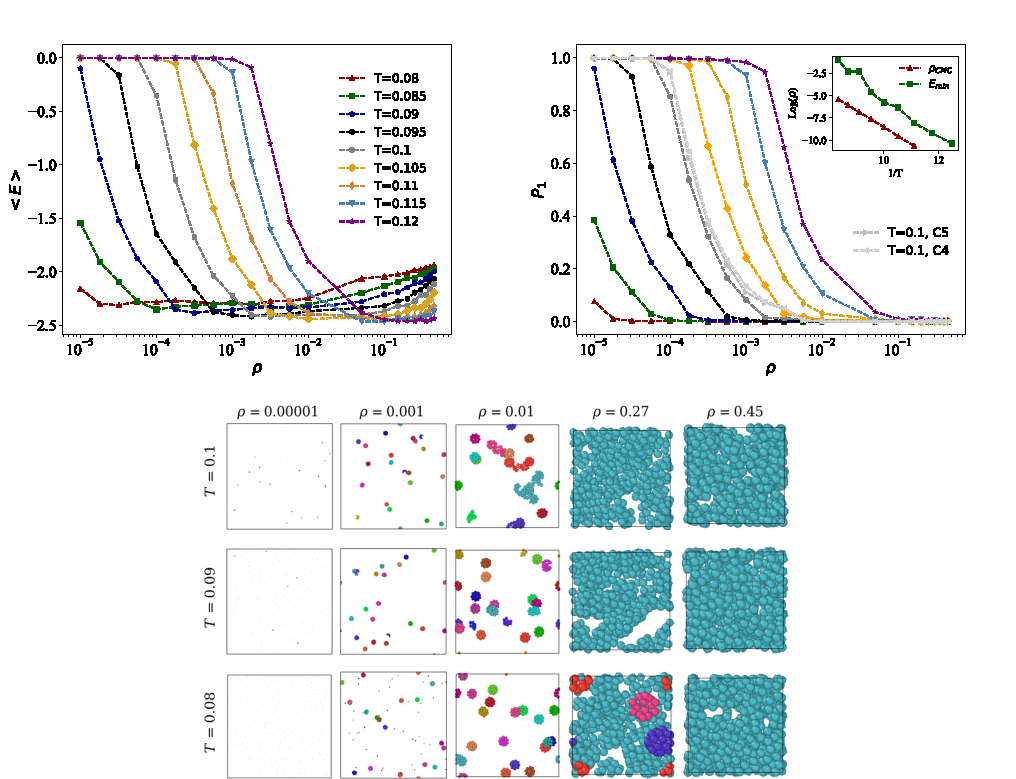
\includegraphics{fig5.pdf}
	\caption{\label{Energy} (Top left) Average potential energy per particle as a function of density for different isotherms. For clarity, the x-axis is in log-scale. We observe a non monotonic behaviour of the average energy characteristic of self-assembly systems. (Top right) Fraction of monomers as a function of the density. Two new curves were added at $T=0.1$, with a different solution (as shown in Fig.~\ref{Yield}). The inset shows the point at which the fraction of monomers is equal to $50\%$ (critical micelle concentration) as a function of the inverse temperature. On the bottom are shown frontal snapshots of the system for different densities and temperatures. Images were obtained with OVITO, where the colors represent particles that belong to the same cluster. For low densities, some colors repeat themselves even though particles are not bounded due to the large number of unbounded particles which count as clusters of size one. All results were simulated with the one specie and two color design (except for the two curves in the top right plot), with an in plane angle of $90$ degrees and a $\cos\theta_{max}=0.98$.}
\end{figure*}

\subsection{Thermodynamic properties}

Given the simplicity of the two color solution, C2(1), we also present a simple study of the phase behavior of this patchy particles in Fig.~\ref{Energy}. As a first approach we restrict ourselves to the parameters $\cos\theta_{max}=0.98$ and an in plane angle of $90$ degrees. This combination favors the snub cube shell as presented above. We observe a non-monotonic behavior of the average energy as a function of density, characteristic of self-assembly systems \cite{Sciortino2009}. For low densities there is an entropic gas phase where most particles are unbounded. As density increases or temperature decreases, more clusters will be formed. For intermediate densities we observe the minimum of the energy which corresponds to a gas of snub cubes. Here, the density is large enough and the temperature low enough for particles to bound and remain bounded until a snub cube is formed. These shells are the equilibrium structures for the patchy particles used which leads to the gas of clusters. For large densities, the liquid phase is approached and less clusters are formed leading to an increase of the average energy. Eventually the liquid phase percolates the system. These results in combination with the snapshots shown suggest there is a possible phase separation of the liquid and gas phase. Future studies should focus on the characterization of the phase space of these structures.

The right plot of Fig.~\ref{Energy} shows the fractions of monomers as a functions of density. All the same temperatures are shown as the plot on the left, but two new curves are added at $T=0.1$ with designs C4(1) and C5 (see Fig.~\ref{Yield}). We find that the behavior for lower densities is similar independently of the design used; it becomes relevant only at higher densities. This suggests that mean field theories, like Wertheim theory \cite{Chapman1989}, might be able to describe these systems at low densities independently of design used. We also measure the critical micelle concentration ($X_{CMC}$), which corresponds to the point where the density of monomers is $50\%$. Using a linear interpolation of the points we reach the values shown in the inset of Fig.~\ref{Energy}. We also plot the logarithm of the critical micelle concentration as a function of the inverse temperature in the inset, highlighting the linear dependence. This is in line with the theoretical predictions for other systems \cite{israelachvili2011}, suggesting a possible extension of the theory to the shells explored here.

\subsection{Two particle species design}

Lastly, we focus on a more complex design with two species and five colors. In this case we force SAT to calculate a solution that only satisfies one of the structures of Fig.~\ref{SAT}. Figure \ref{Sol} shows the results with the corresponding design. Using SAT it is possible to generate solutions which exclude specific structures. Thus, one can, for example, calculate a solution that satisfies the topological constraints of the icosahedron but does not of the snub cube or snub dodecahedron. With this method, we prove that one can not only increase the range of parameters where a certain shell is formed but we also increase its yield, since it is more rare to find competing structures. Both for the icosahedron and snub cube designs we observe the increase of the parameter ranges over more in plane angles as well as $\cos\theta_{max}$, meaning that they are more resilient to changes in the geometry of the patches and width of the interactions. On the other hand, the diagram of the snub dodecahedron does not change substantially when compared to Fig~\ref{N1c2}. In this case, although the two species and five colors solution only satisfies the snub dodecahedron, one of the species, by itself, is able to form the other competing shells. We hypothesize that this will always be the case for any design, since the topology of the snub dodecahedron is almost the same as the snub cube, in term of which bonds are formed between particles and their orientations. Only one particle is the exception which is necessary to close the snub dodecahedron and not the snub cube. Thus, in any design with more than one species that satisfies the snub dodecahedron, there might be a subset of those species that will always satisfy the snub cube as well. We have explored all solutions in the two species case, varying the number of colors from two to ten, and in all one of its subsets always satisfies other shells (icosahedron or snub cube). One could try to exhaust (by brute force) all possible species and color combinations but as species and colors increase so do the number of solutions (and its subsets) making this a very demanding task.

\begin{figure*}[t]
	\includegraphics{fig6.pdf}
	\caption{\label{Sol} Most probable structure formed for different in plane angles of $\textbf{p}_4$ and $\textbf{p}_5$ in Eq.~\ref{patch} and for different patch width, $\cos\theta_{max}$, in Eq.~\ref{KF}. Here, each shell if formed using a two species and five colors design which only satisfies each of the structures shown. On the left the design only satisfies the icosahedron, in the middle the snub cube and on the right the snub dodecahedron. In the last plot all the shells are formed even though the design only satisfies the snub dodecahedron. This is because one single particle specie is enough to form the other structures.}
\end{figure*}

\section{Conclusion}

In this work we have shown how to translate the self-assembly of finite-size structures using patchy particles into a SAT problem. Using patchy particles of valence five we explored different structures through Monte Carlo simulations and how to optimize the parameters to enhance self-assembly. We have proved that doing the most trivial design of patchy particles (one specie and one color) is worse than using SAT. While the most trivial design only yields one of the possible three shells, by slightly increasing the complexity of the design (adding one color) and allowing SAT to color the patches we find an overall improvement. The SAT design not only increases the probability of forming the finite size structures but allows us to explore different structures. Thus, we show that with these patchy particles one can form the icosahedron, snub cube or snub dodecahedron. We also show how these structures are affected by density, showing that larger structures are harder to assemble in higher densities and smaller ones, like the icosahedron, are favored due to their small size leading to an increase in yield.

We also explored the phase diagram of these patchy particles designed with SAT. We find a non-monotonous behavior of the average potential energy as a function of density, as is typical of self-assembly systems \cite{Sciortino2009}. These results suggest a first entropic gas phase at very low densities, followed by a gas phase of clusters near the energy minima, ending at the liquid phase at high densities. Our results suggest the existence of a liquid-gas coexistence region. Future studies should focus on a systematic study of the phase diagram. We also measured the critical miscelle concentration for this system and found it goes in line with previous theoretical results. Here, we show a comparison between different particle designs and conclude that the difference is not significant. This suggests that mean-field theories that do not take these details into account might still be successful in describing them.

Lastly, we used SAT to target only one of the structures previously assembled. For this, we increased the complexity of the design to two particle species and five patch colors. We use SAT to calculate particle designs that only satisfy one of the structures while excluding the others. We observe that for the icosahedron and snub cube, the designs obtained only satisfy these structures. Due to that the yield increases and we also find a wider parameter range where it is possible to successfully assemble these structures. The snub cube and icosahedron can reach yields of almost $100\%$, while the snub dodecahedron can reach approximately $50\%$, on average. While it is possible to find a design that only satisfies the snub dodecahedron, all of its subsets do not. Thus, one of the particle species, by itself, can always assemble one (or both) of the other structures. This results in a diagram of assembled structures which is similar to the previous one specie and two colors. We argue that this happens due to the topology of the snub dodecahedron. It is always possible to take a subset of particles of this structure to form the other ones. Although we are not aware of an exact prove, our results suggest it. We find no solutions in the two species case (and colors varying from two to ten) that satisfies the snub dodecahedron, where any subset of it does not satisfy the others. One could try to brute force higher particle species but this also increases the number of solutions that need to be tested making it a very demanding task.

Although we have only shown results for patchy particles of valence five, we have been able to successfully assemble other structures with different valences. It would be interesting to explore if similar permutations between structures is possible in other valences. With fewer patches the structures will need more parameter optimization to assemble since the number of bonds per particle is fewer and thus the structures can be less stable while forming. This might increase the probability of being stuck in kinetic traps.

One of the possible pathways of realizing these designs experimentally is through 3D DNA nanomaterials, in particular wireframe DNA origami. Previous studies have successfully shown the versatility of these building blocks in assembling a wide array of structures \cite{Mosayebi2017, Lee2022, Jun2021, Rothemund2006}. Furthermore, through the use of complementary strands one can functionalize the wireframe to act as a patchy particle with selective spatial bonding and tune the interactions accordingly \cite{Biancaniello2005, Wang2015}. We also argue that our results support such approach not only due to the high yields observed in simulations, but also due to the robustness of the structures formed to flexibility of the bonds, which is characteristic of DNA bonds \cite{Meulen2015, Meulen2015, Geerts2010}.

A demanding question would be to find a way to predict which design is better when using SAT. One of the gaps in this formulation is that there is no apriori knowledge which structures can form for a given SAT design. This comes only from intuition or after testing a given design in simulations. This requires a feedback loop between SAT and simulations that can be quite demanding, depending on the number of possible structures formed with the same design. Thus, finding apriori which designs generate configurations with the lowest energy would be of interest to not only self-assembly but also many other fields that deal with complex and disordered systems \cite{Franz2017}.

SAT has already been applied as an inverse assembly tool to form crystals and now in finite-size structures. This proves the resilience of SAT for self-assembly problems. Future studies will also focus on exploring other possible materials and structures that so far have been quite challenging to assemble. For example, SAT can become a useful tool in the assembly of quasi-crystals where the lack of translation symmetry (unlike the crystal) makes the assembly process a daunting task \cite{Shechtman1984}. Recent studies have managed to simulate patchy particle systems which are able form quasi-crystals \cite{Noya2021}. Unfortunately, there is still a large degree of complexity in choosing the optimal design for targeting specific quasi-crystals, making it difficult to systematically change between structures without doing demanding simulation work first that is highly based on trial and error. SAT can help in this front, by creating a consistent algorithm that can find the appropriate design to target the specific structure without any previous trial and error task.

\section{Acknowledgements}

The authors acknowledge all the financial support from the European Research Council Grant DLV-759187.

\bibliography{refs}

\end{document}
